\documentclass[main.tex]{subfiles}
\begin{document}
\section{Bài 6}

\newcommand{\U}{\ensuremath{\mathcal U} }
\newcommand{\A}[1]{\ensuremath{A_{#1}}}
\newcommand{\x}[1]{\ensuremath{x_{#1}}}
\newcommand{\abs}[1]{\ensuremath{\left|#1\right|}}
\newcommand{\ssum}[3]{\sum_{#1}^{#2}{#3}}
\newcommand{\vv}{\dots}

\begin{wrapfigure}{L}{0.25\textwidth}
\centering
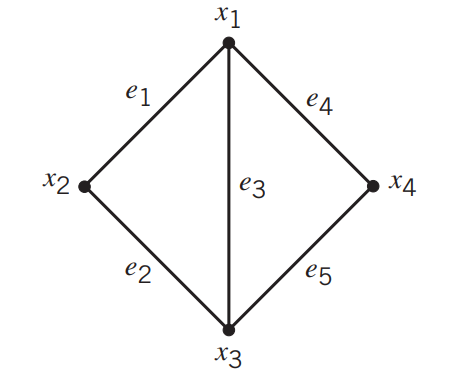
\includegraphics[width=0.25\textwidth]{image/Bai6.png}
\captionsetup{labelformat=empty}
\caption{(G)}
\vspace*{-1cm}
\end{wrapfigure}

- Gọi \U là các cách tô $n$ màu cho 4 đỉnh của đồ thị (G).\\
- Do (G) có 4 đỉnh, mỗi đỉnh có $n$ cách tô màu nên theo nguyên lý nhân, số cách tô màu cho 4 đỉnh của (G) là $n^4$.\\
- Gọi \A 1, \A 2, \A 3, \A 4, \A 5 lần lượt là tập các cách tô màu cho 2 đỉnh kề với các cạnh $e_1, e_2, e_3, e_4, e_5$ sao cho 2 đỉnh kề với $e_i$ luôn có cùng màu. Như vậy số cách tô $n$ màu sao cho không có 2 đỉnh kề nào cùng màu là$\overline{\A1\A2\A3\A4\A5}$\\ \\

\paragraph*{Tính $S_1$}
\begin{wrapfigure}{R}{0.25\textwidth}
\centering
\vspace*{-1cm}
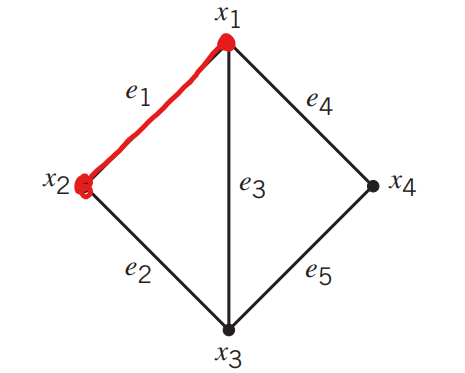
\includegraphics[width=0.25\textwidth]{image/Bai6_S1.png}
\captionsetup{labelformat=empty}
\caption{\textit{Tô màu cho 1 cạnh}}
\vspace*{-1cm}
\end{wrapfigure}

Ta xét \abs{\A 1}: ta có $n$ cách tô màu cho 2 đỉnh kề với $e_1$ và $n^2$ cách cho 2 đỉnh còn lại $\Rightarrow \abs{\A 1} = n^3$ (nguyên lý nhân).\\
Lý luận tương tự, ta cũng có \A 2 = \A 3 = \A 4 = \A 5 = $n^3$.\\ 
Vậy, $S_1 = 5n^3$.\\ 

\paragraph*{Tính $S_2$}
\begin{wrapfigure}{R}{0.25\textwidth}
\centering
\vspace*{-1cm}
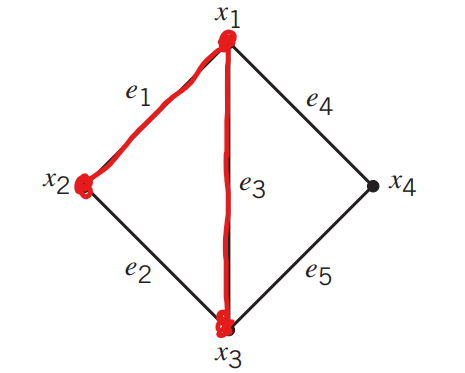
\includegraphics[width=0.25\textwidth]{image/Bai6_S2.png}
\captionsetup{labelformat=empty}
\caption{\textit{Tô màu cho 2 cạnh}}
\vspace*{-1cm}

\end{wrapfigure}

Ta nhận thấy 2 cạnh của (G) luôn nối liền 3 đỉnh nên có $n$ cách tô màu cho 3 đỉnh đó và $n$ cách nữa cho đỉnh còn lại. Vậy theo nguyên lý nhân, $\abs{A_iA_j}=n^2$.\\
- Suy ra $S_2 = {5 \choose 2} n^2$. \\


\paragraph*{Tính $S_3$}
Xét \abs{A_1A_2A_3}: ta thấy $e_1,\ e_2,\ e_3$ nối liền 3 đỉnh \x1, \x2, \x3 nên ta có $n$ cách tô màu cho 3 đỉnh này, và $n$ cách nữa cho đỉnh còn lại nên $\abs{A_1A_2A_3} = n^2$.\\
- Xét \abs{A_3A_4A_5}: ta thấy $e_3,\ e_4,\ e_5$ nối liền 3 đỉnh \x1, \x4, \x3 nên tương tự như trên, ta có $\abs{A_3A_4A_4} = n^2$.\\ 
- Với \abs{A_iA_jA_k} với các $(i,j,k) \neq (1, 2, 3) \neq (3, 4, 5)$ thì 3 cạnh $e_i,\ e_j,\ e_k$ luôn nối liền cả 4 đỉnh của (G).\\
Ta suy ra: 
$$
S_3 = 2n^2 - \left[{5\choose3}-2\right]n = 2n^2+8n
$$
\begin{figure}[H]
\centering
\begin{minipage}{0.25\textwidth}
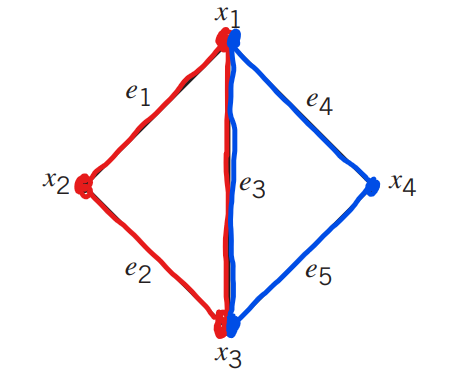
\includegraphics[width=\textwidth]{image/Bai6_S3_1.png}
\captionsetup{labelformat=empty}
\caption{\abs{A_1A_2A_3} và \abs{A_3A_4A_5}}
\end{minipage}
\begin{minipage}{0.25\textwidth}
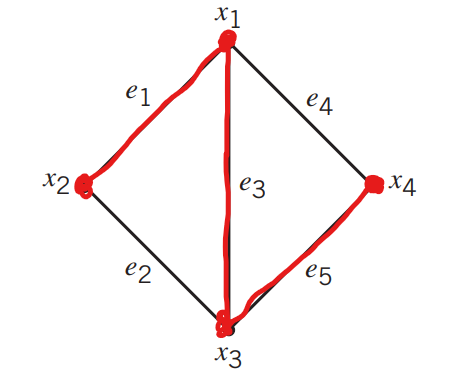
\includegraphics[width=\textwidth]{image/Bai6_S3_2.png}
\captionsetup{labelformat=empty}
\caption{Các TH còn lại}
\end{minipage}
\end{figure}

\paragraph*{Tính $S_4$ và $S_5$} 
Ta nhận thấy 4 hay 5 cạnh bất kì của (G) luôn nối liền 4 đỉnh của nó nên:
\begin{gather*}
S_4 = {5\choose4}n \\
S_5 = n    
\end{gather*}

\begin{figure}[H]
\centering
\begin{minipage}{0.25\textwidth}
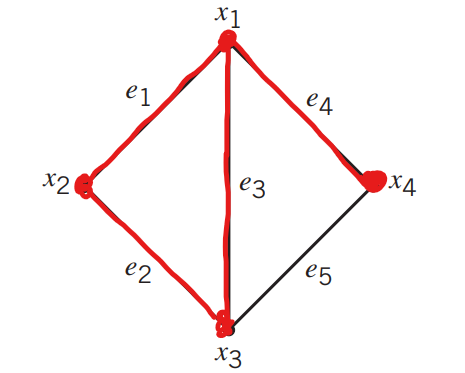
\includegraphics[width=\textwidth]{image/Bai6_S4.png}
\captionsetup{labelformat=empty}
\caption{4 cạnh}
\end{minipage}
\begin{minipage}{0.25\textwidth}
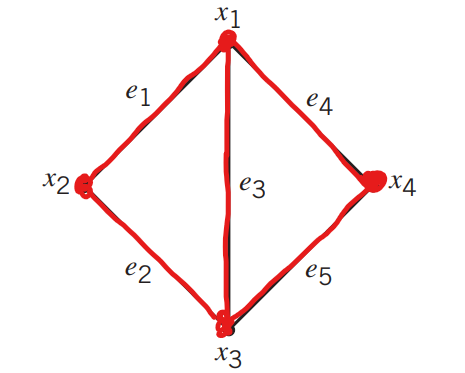
\includegraphics[width=\textwidth]{image/Bai6_S5.png}
\captionsetup{labelformat=empty}
\caption{5 cạnh}
\end{minipage}
\end{figure}

\paragraph*{Vậy theo nguyên lý bù trừ} 
\begin{align*}
\abs{\overline{A_1A_2A_3A_4A_5}} &= \abs{\U} - S_1 + S_2 - S_3 + S_4 - S_5\\
&= n^4 - 5n^3 + {5\choose2}n^2-(2n^2+8n)+{5\choose4}n-n\\
&= n^4 - 5n^3 + 10n^2 - (2n^2+8n) + 5n - n\\
&= n^4 - 5n^3 + 8n^2 - 4n
\end{align*}


\end{document}